\section{Lecture 6: Kalman Filter, Observability Analysis, and KF-Based VINS}
\label{sec:lecture06}

\paragraph{Topics.} (1) the MAP problem behind the Kalman filter; (2) linearization of the MAP problem; (3) Solution 1: solve it incrementally --- the (E)KF; (4) Solution 2: solve it by batch; (5) discussion: the EKF, MLE/MAP, and the VINS system; (6) visual-inertial initialization.

% Tighten matrix column spacing for the block-matrix algebra in this lecture.
\setlength{\arraycolsep}{3.5pt}

% =====================================================================
\subsection{The MAP problem behind the Kalman filter}
\label{sec:lec06-map}

The Kalman filter (KF) is a \emph{linear} estimator based on the \emph{Gaussian} assumption. Before deriving it, let's first start with a MAP problem. Given
\begin{empheq}[box=\fbox]{align}
\begin{cases}
\vect{x}_0 \sim \mathcal{N}(\hat{\vect{x}}_0, \vect{P}_0) & \to\; \text{prior}, \\[2pt]
\vect{x}_1 = \vect{f}(\vect{x}_0) + \vect{w}_0, \quad \vect{w}_0 \sim \mathcal{N}(\vect{0}, \vect{Q}_0) & \to\; \text{motion model (IMU)}, \\[2pt]
\vect{z}_1 = \vect{h}(\vect{x}_1) + \vect{n}_1, \quad\; \vect{n}_1 \sim \mathcal{N}(\vect{0}, \vect{R}) & \to\; \text{measurement model (vision)},
\end{cases}
\label{eq:lec06-system}
\end{empheq}
the target is the posterior distribution of the new state:
\begin{align}
\vect{x}_1 \sim \mathcal{N}(\hat{\vect{x}}_1, \vect{P}_1).
\end{align}

\paragraph{How to compute it?} With $\vect{x} = \{\vect{x}_0, \vect{x}_1\}$ and $\vect{z} = \vect{z}_1$, apply Bayes' rule and factorize:
\begin{align}
\max_{\vect{x}}\; p(\vect{x}|\vect{z})
&= \max_{\vect{x}}\; \frac{p(\vect{z}|\vect{x})\,p(\vect{x})}{p(\vect{z})}
= \max_{\vect{x}}\; \frac{p(\vect{z}_1|\vect{x}_1,\vect{x}_0)\,p(\vect{x}_1,\vect{x}_0)}{p(\vect{z}_1)} \\
&= \max_{\vect{x}}\; \frac{p(\vect{z}_1|\vect{x}_1,\vect{x}_0)\,p(\vect{x}_1|\vect{x}_0)\,p(\vect{x}_0)}{p(\vect{z}_1)} \\
&= \max_{\vect{x}}\; \frac{p(\vect{z}_1|\vect{x}_1)\,p(\vect{x}_1|\vect{x}_0)\,p(\vect{x}_0)}{p(\vect{z}_1)},
\end{align}
where in the last step $\vect{z}_1$ only depends on $\vect{x}_1$, so we drop $\vect{x}_0$ from the measurement factor. Taking the negative log-likelihood of the three Gaussian factors (and recalling $\norm{\vect{e}}^2_{\vect{P}} \triangleq \vect{e}\trans\vect{P}^{-1}\vect{e}$), the MAP problem is equivalent to
\begin{empheq}[box=\fbox]{align}
\min_{\vect{x}}\;
\norm{\vect{z}_1 - \vect{h}(\vect{x}_1)}^2_{\vect{R}}
+ \norm{\vect{x}_1 - \vect{f}(\vect{x}_0)}^2_{\vect{Q}_0}
+ \norm{\vect{x}_0 - \hat{\vect{x}}_0}^2_{\vect{P}_0}.
\label{eq:lec06-map-cost}
\end{empheq}

% =====================================================================
\subsection{Linearization}
\label{sec:lec06-lin}

Stack the state and choose the linearization point:
\begin{align}
\vect{x} = \begin{bmatrix} \vect{x}_0 \\ \vect{x}_1 \end{bmatrix},
\qquad
\text{linearization point:}\;\;
\hat{\vect{x}} = \begin{bmatrix} \hat{\vect{x}}_0 \\ \hat{\vect{x}}_1 \end{bmatrix},
\qquad
\tilde{\vect{x}} = \vect{x} - \hat{\vect{x}}.
\end{align}

\paragraph{Motion model.} From $\vect{x}_1 = \vect{f}(\vect{x}_0) + \vect{w}_0$, linearizing $\vect{f}$ at $\hat{\vect{x}}_0$ with Jacobian $\vect{F}$,
\begin{align}
\hat{\vect{x}}_1 + \tilde{\vect{x}}_1 \approx \vect{f}(\hat{\vect{x}}_0) + \vect{F}\,(\vect{x}_0 - \hat{\vect{x}}_0) + \vect{w}_0
= \vect{f}(\hat{\vect{x}}_0) + \vect{F}\,\tilde{\vect{x}}_0 + \vect{w}_0.
\end{align}
Define the \emph{motion residual} $\vect{r}_x$:
\begin{align}
\vect{r}_x \triangleq \hat{\vect{x}}_1 - \vect{f}(\hat{\vect{x}}_0)
= \vect{F}\,\tilde{\vect{x}}_0 - \tilde{\vect{x}}_1 + \vect{w}_0
= \begin{bmatrix} \vect{F} & -\vect{I} \end{bmatrix}
\begin{bmatrix} \tilde{\vect{x}}_0 \\ \tilde{\vect{x}}_1 \end{bmatrix} + \vect{w}_0.
\label{eq:lec06-rx}
\end{align}

\paragraph{Measurement model.} From $\vect{z}_1 = \vect{h}(\vect{x}_1) + \vect{n}_1$, linearizing $\vect{h}$ at $\hat{\vect{x}}_1$ with Jacobian $\vect{H}$,
\begin{align}
\vect{z}_1 = \vect{h}(\hat{\vect{x}}_1) + \vect{H}\,(\vect{x}_1 - \hat{\vect{x}}_1) + \vect{n}_1
\;\;\Rightarrow\;\;
\tilde{\vect{z}}_1 \triangleq \vect{z}_1 - \vect{h}(\hat{\vect{x}}_1)
= \vect{H}\,\tilde{\vect{x}}_1 + \vect{n}_1
= \begin{bmatrix} \vect{0} & \vect{H} \end{bmatrix}
\begin{bmatrix} \tilde{\vect{x}}_0 \\ \tilde{\vect{x}}_1 \end{bmatrix} + \vect{n}_1.
\label{eq:lec06-zres}
\end{align}

\paragraph{The linearized cost.} Then the cost function \eqref{eq:lec06-map-cost} becomes
\begin{empheq}[box=\fbox]{align}
C = \norm{\tilde{\vect{z}}_1 - \vect{H}\tilde{\vect{x}}_1}^2_{\vect{R}}
+ \norm*{\vect{r}_x - \begin{bmatrix} \vect{F} & -\vect{I} \end{bmatrix}
\begin{bmatrix} \tilde{\vect{x}}_0 \\ \tilde{\vect{x}}_1 \end{bmatrix}}^2_{\vect{Q}_0}
+ \norm{\tilde{\vect{x}}_0}^2_{\vect{P}_0}.
\label{eq:lec06-lincost}
\end{empheq}

% =====================================================================
\subsection{Solution 1: solve it incrementally --- the (E)KF}
\label{sec:lec06-incremental}

Solve \eqref{eq:lec06-lincost} in two steps:
\begin{align}
\begin{cases}
\text{step 1:} \quad
\norm{\tilde{\vect{x}}_0}^2_{\vect{P}_0}
+ \norm*{\vect{r}_x - \begin{bmatrix} \vect{F} & -\vect{I} \end{bmatrix}
\begin{bmatrix} \tilde{\vect{x}}_0 \\ \tilde{\vect{x}}_1 \end{bmatrix}}^2_{\vect{Q}_0}
& \to\quad \vect{x}_{1|0} \sim \mathcal{N}(\hat{\vect{x}}_{1|0}, \vect{P}_{1|0}), \\[10pt]
\text{step 2:} \quad
\norm{\tilde{\vect{x}}_{1|0}}^2_{\vect{P}_{1|0}}
+ \norm{\tilde{\vect{z}}_1 - \vect{H}\tilde{\vect{x}}_1}^2_{\vect{R}}
& \to\quad \vect{x}_{1|1} \sim \mathcal{N}(\hat{\vect{x}}_{1|1}, \vect{P}_{1|1}).
\end{cases}
\end{align}

\paragraph{Step 1: prior + motion.} We solve
\begin{align}
\min_{\tilde{\vect{x}}}\;
\norm{\tilde{\vect{x}}_0}^2_{\vect{P}_0}
+ \norm*{\vect{r}_x - \begin{bmatrix} \vect{F} & -\vect{I} \end{bmatrix}
\begin{bmatrix} \tilde{\vect{x}}_0 \\ \tilde{\vect{x}}_1 \end{bmatrix}}^2_{\vect{Q}_0}.
\end{align}
Expanding, the cost is
\begin{align}
C_1 =
\begin{bmatrix} \tilde{\vect{x}}_0 \\ \tilde{\vect{x}}_1 \end{bmatrix}\trans
\begin{bmatrix}
\vect{P}_0^{-1} + \vect{F}\trans\vect{Q}_0^{-1}\vect{F} & -\vect{F}\trans\vect{Q}_0^{-1} \\
-\vect{Q}_0^{-1}\vect{F} & \vect{Q}_0^{-1}
\end{bmatrix}
\begin{bmatrix} \tilde{\vect{x}}_0 \\ \tilde{\vect{x}}_1 \end{bmatrix}
- 2 \begin{bmatrix} \tilde{\vect{x}}_0 \\ \tilde{\vect{x}}_1 \end{bmatrix}\trans
\begin{bmatrix} \vect{F}\trans \\ -\vect{I} \end{bmatrix} \vect{Q}_0^{-1}\,\vect{r}_x
+ \vect{r}_x\trans\vect{Q}_0^{-1}\vect{r}_x.
\end{align}
Setting $\frac{\partial C_1}{\partial \left[\begin{smallmatrix} \tilde{\vect{x}}_0 \\ \tilde{\vect{x}}_1 \end{smallmatrix}\right]} = \vect{0}$ gives the \emph{information system}:
\begin{align}
\begin{bmatrix}
\vect{P}_0^{-1} + \vect{F}\trans\vect{Q}_0^{-1}\vect{F} & -\vect{F}\trans\vect{Q}_0^{-1} \\
-\vect{Q}_0^{-1}\vect{F} & \vect{Q}_0^{-1}
\end{bmatrix}
\begin{bmatrix} \tilde{\vect{x}}_0 \\ \tilde{\vect{x}}_1 \end{bmatrix}
=
\begin{bmatrix} \vect{F}\trans\vect{Q}_0^{-1}\,\vect{r}_x \\ -\vect{Q}_0^{-1}\,\vect{r}_x \end{bmatrix}.
\label{eq:lec06-infosys1}
\end{align}
Then, marginalizing $\tilde{\vect{x}}_0$ (Schur complement onto the $\tilde{\vect{x}}_1$ block, Lecture~4),
\begin{align}
\Big[ \vect{Q}_0^{-1} - \vect{Q}_0^{-1}\vect{F}\big(\vect{P}_0^{-1} + \vect{F}\trans\vect{Q}_0^{-1}\vect{F}\big)^{-1}\vect{F}\trans\vect{Q}_0^{-1} \Big] \tilde{\vect{x}}_1
= -\vect{Q}_0^{-1}\,\vect{r}_x + \vect{Q}_0^{-1}\vect{F}\big(\vect{P}_0^{-1} + \vect{F}\trans\vect{Q}_0^{-1}\vect{F}\big)^{-1}\vect{F}\trans\vect{Q}_0^{-1}\,\vect{r}_x,
\end{align}
and applying the matrix inversion lemma to both sides,
\begin{align}
\underbrace{\big(\vect{Q}_0 + \vect{F}\vect{P}_0\vect{F}\trans\big)^{-1}}_{\vect{P}_{1|0}^{-1}} \tilde{\vect{x}}_1
= -\big(\vect{Q}_0 + \vect{F}\vect{P}_0\vect{F}\trans\big)^{-1}\,\vect{r}_x.
\end{align}
Hence
\begin{empheq}[box=\fbox]{align}
\tilde{\vect{x}}_1 = -\vect{r}_x,
\qquad
\vect{P}_{1|0} = \vect{Q}_0 + \vect{F}\vect{P}_0\vect{F}\trans.
\label{eq:lec06-step1}
\end{empheq}
Interpreting $\tilde{\vect{x}}_1 = -\vect{r}_x$:
\begin{align}
\begin{cases}
\text{if } \vect{r}_x = \vect{0}, & \hat{\vect{x}}_{1|0} = \vect{f}(\hat{\vect{x}}_0), \\
\text{if } \vect{r}_x \neq \vect{0}, & \hat{\vect{x}}_{1|0} = \vect{f}(\hat{\vect{x}}_0) - \vect{r}_x.
\end{cases}
\end{align}

\paragraph{Step 2: + update.} Since step~1 left $\tilde{\vect{x}}_1$ with mean $-\vect{r}_x$ and covariance $\vect{P}_{1|0}$, the remaining problem is
\begin{align}
\min_{\tilde{\vect{x}}_1}\;
\norm{\tilde{\vect{x}}_1 + \vect{r}_x}^2_{\vect{P}_{1|0}}
+ \norm{\tilde{\vect{z}}_1 - \vect{H}\tilde{\vect{x}}_1}^2_{\vect{R}}.
\end{align}
Expanding (one step per row, dropping the tilde-$1$ subscript on $\tilde{\vect{z}}$ for brevity):
\begin{align}
C_2 &= (\tilde{\vect{x}}_1 + \vect{r}_x)\trans\vect{P}_{1|0}^{-1}(\tilde{\vect{x}}_1 + \vect{r}_x)
+ (\tilde{\vect{z}} - \vect{H}\tilde{\vect{x}}_1)\trans\vect{R}^{-1}(\tilde{\vect{z}} - \vect{H}\tilde{\vect{x}}_1) \\
&= \tilde{\vect{x}}_1\trans\vect{P}_{1|0}^{-1}\tilde{\vect{x}}_1
+ 2\,\tilde{\vect{x}}_1\trans\vect{P}_{1|0}^{-1}\vect{r}_x
+ \vect{r}_x\trans\vect{P}_{1|0}^{-1}\vect{r}_x
+ \tilde{\vect{z}}\trans\vect{R}^{-1}\tilde{\vect{z}}
- 2\,\tilde{\vect{z}}\trans\vect{R}^{-1}\vect{H}\tilde{\vect{x}}_1
+ \tilde{\vect{x}}_1\trans\vect{H}\trans\vect{R}^{-1}\vect{H}\tilde{\vect{x}}_1 \\
&= \tilde{\vect{x}}_1\trans\big(\vect{P}_{1|0}^{-1} + \vect{H}\trans\vect{R}^{-1}\vect{H}\big)\tilde{\vect{x}}_1
+ 2\,\tilde{\vect{x}}_1\trans\big(\vect{P}_{1|0}^{-1}\vect{r}_x - \vect{H}\trans\vect{R}^{-1}\tilde{\vect{z}}\big)
+ \tilde{\vect{z}}\trans\vect{R}^{-1}\tilde{\vect{z}}
+ \vect{r}_x\trans\vect{P}_{1|0}^{-1}\vect{r}_x.
\end{align}
Hence, $\frac{\partial C_2}{\partial \tilde{\vect{x}}_1} = \vect{0}$ gives
\begin{align}
\underbrace{\big(\vect{P}_{1|0}^{-1} + \vect{H}\trans\vect{R}^{-1}\vect{H}\big)}_{\vect{\Sigma}\,=\,\vect{P}_{1|1}^{-1}}\,\tilde{\vect{x}}_1
= \vect{H}\trans\vect{R}^{-1}\tilde{\vect{z}} - \vect{P}_{1|0}^{-1}\,\vect{r}_x,
\label{eq:lec06-update-normal}
\end{align}
so that
\begin{align}
\tilde{\vect{x}}_1
&= \big(\vect{P}_{1|0}^{-1} + \vect{H}\trans\vect{R}^{-1}\vect{H}\big)^{-1}\big(\vect{H}\trans\vect{R}^{-1}\tilde{\vect{z}} - \vect{P}_{1|0}^{-1}\vect{r}_x\big) \\
&= \big(\vect{P}_{1|0}^{-1} + \vect{H}\trans\vect{R}^{-1}\vect{H}\big)^{-1}\vect{H}\trans\vect{R}^{-1}\tilde{\vect{z}}
- \big(\vect{P}_{1|0}^{-1} + \vect{H}\trans\vect{R}^{-1}\vect{H}\big)^{-1}\vect{P}_{1|0}^{-1}\vect{r}_x.
\label{eq:lec06-xtilde-two-terms}
\end{align}

\paragraph{The gain equivalence.} For the first term of \eqref{eq:lec06-xtilde-two-terms}, apply the matrix inversion lemma, $\big(\vect{P}_{1|0}^{-1} + \vect{H}\trans\vect{R}^{-1}\vect{H}\big)^{-1} = \vect{P}_{1|0} - \vect{P}_{1|0}\vect{H}\trans\big(\vect{H}\vect{P}_{1|0}\vect{H}\trans + \vect{R}\big)^{-1}\vect{H}\vect{P}_{1|0}$, and simplify step by step:
\begin{align}
&\Big(\vect{P}_{1|0} - \vect{P}_{1|0}\vect{H}\trans\big(\vect{H}\vect{P}_{1|0}\vect{H}\trans + \vect{R}\big)^{-1}\vect{H}\vect{P}_{1|0}\Big)\vect{H}\trans\vect{R}^{-1}\,\tilde{\vect{z}} \notag \\
&= \Big(\vect{P}_{1|0}\vect{H}\trans\vect{R}^{-1} - \vect{P}_{1|0}\vect{H}\trans\big(\vect{H}\vect{P}_{1|0}\vect{H}\trans + \vect{R}\big)^{-1}\vect{H}\vect{P}_{1|0}\vect{H}\trans\vect{R}^{-1}\Big)\,\tilde{\vect{z}} \\
&= \vect{P}_{1|0}\vect{H}\trans\Big(\vect{R}^{-1} - \big(\vect{H}\vect{P}_{1|0}\vect{H}\trans + \vect{R}\big)^{-1}\vect{H}\vect{P}_{1|0}\vect{H}\trans\vect{R}^{-1}\Big)\,\tilde{\vect{z}} \\
&= \vect{P}_{1|0}\vect{H}\trans\big(\vect{H}\vect{P}_{1|0}\vect{H}\trans + \vect{R}\big)^{-1}\Big(\big(\vect{H}\vect{P}_{1|0}\vect{H}\trans + \vect{R}\big)\vect{R}^{-1} - \vect{H}\vect{P}_{1|0}\vect{H}\trans\vect{R}^{-1}\Big)\,\tilde{\vect{z}} \\
&= \vect{P}_{1|0}\vect{H}\trans\big(\vect{H}\vect{P}_{1|0}\vect{H}\trans + \vect{R}\big)^{-1}\,\tilde{\vect{z}}.
\label{eq:lec06-gain-equiv}
\end{align}
Hence we got
\begin{empheq}[box=\fbox]{align}
\tilde{\vect{x}}_1 = \vect{P}_{1|0}\vect{H}\trans\big(\vect{H}\vect{P}_{1|0}\vect{H}\trans + \vect{R}\big)^{-1}\,\tilde{\vect{z}}
- \big(\vect{P}_{1|0}^{-1} + \vect{H}\trans\vect{R}^{-1}\vect{H}\big)^{-1}\vect{P}_{1|0}^{-1}\,\vect{r}_x.
\label{eq:lec06-update}
\end{empheq}
If $\vect{r}_x \to \vect{0}$, then
\begin{align}
\tilde{\vect{x}}_1 = \vect{P}_{1|0}\vect{H}\trans\big(\vect{H}\vect{P}_{1|0}\vect{H}\trans + \vect{R}\big)^{-1}\,\tilde{\vect{z}},
\end{align}
and the posterior covariance follows from \eqref{eq:lec06-update-normal} (matrix inversion lemma again):
\begin{align}
\vect{P}_{1|1} = \big(\vect{P}_{1|0}^{-1} + \vect{H}\trans\vect{R}^{-1}\vect{H}\big)^{-1}
= \vect{P}_{1|0} - \vect{P}_{1|0}\vect{H}\trans\big(\vect{H}\vect{P}_{1|0}\vect{H}\trans + \vect{R}\big)^{-1}\vect{H}\vect{P}_{1|0}.
\end{align}
Therefore, we have the posterior $\vect{x}_{1|1} \sim \mathcal{N}(\hat{\vect{x}}_{1|1}, \vect{P}_{1|1})$.

\paragraph{Summary of the process.} Collecting the two steps ($\vect{r}_x \to \vect{0}$):
\begin{empheq}[box=\fbox]{align}
&\text{prior:} && \vect{x}_0 \sim \mathcal{N}(\hat{\vect{x}}_0, \vect{P}_0), \notag \\[2pt]
&\text{propagation:} && \vect{x}_1 = \vect{f}(\vect{x}_0) + \vect{w}_0, \notag \\
& && \hat{\vect{x}}_{1|0} = \vect{f}(\hat{\vect{x}}_0), \qquad
\vect{P}_{1|0} = \vect{F}\vect{P}_0\vect{F}\trans + \vect{Q}_0, \notag \\[2pt]
&\text{update:} && \vect{z}_1 = \vect{h}(\vect{x}_1) + \vect{n}_1, \notag \\
& && \tilde{\vect{z}}_1 = \vect{z}_1 - \vect{h}(\hat{\vect{x}}_{1|0}), \qquad
\tilde{\vect{z}}_1 = \vect{H}\tilde{\vect{x}}_1 + \vect{n}_1, \notag \\
& && \vect{S}_1 = \vect{H}\vect{P}_{1|0}\vect{H}\trans + \vect{R}
\quad \to\; \text{innovation covariance}, \label{eq:lec06-kf} \\
& && \vect{K} = \vect{P}_{1|0}\vect{H}\trans\vect{S}_1^{-1}
\quad \to\; \text{Kalman gain}, \notag \\
& && \hat{\vect{x}}_{1|1} = \hat{\vect{x}}_{1|0} + \vect{K}\,\tilde{\vect{z}}_1, \notag \\
& && \vect{P}_{1|1} = \vect{P}_{1|0} - \vect{P}_{1|0}\vect{H}\trans\vect{S}_1^{-1}\vect{H}\vect{P}_{1|0}. \notag
\end{empheq}
\textbf{This is the EKF from the MLE/MAP formulation.}

% =====================================================================
\subsection{Solution 2: solve it by batch}
\label{sec:lec06-batch}

Alternatively, solve the full linearized cost \eqref{eq:lec06-lincost} in one shot. Setting the gradient with respect to $[\tilde{\vect{x}}_0; \tilde{\vect{x}}_1]$ to zero now includes the measurement term in the information system:
\begin{align}
\begin{bmatrix}
\vect{P}_0^{-1} + \vect{F}\trans\vect{Q}_0^{-1}\vect{F} & -\vect{F}\trans\vect{Q}_0^{-1} \\
-\vect{Q}_0^{-1}\vect{F} & \vect{Q}_0^{-1} + \vect{H}\trans\vect{R}^{-1}\vect{H}
\end{bmatrix}
\begin{bmatrix} \tilde{\vect{x}}_0 \\ \tilde{\vect{x}}_1 \end{bmatrix}
=
\begin{bmatrix} \vect{F}\trans\vect{Q}_0^{-1}\,\vect{r}_x \\ -\vect{Q}_0^{-1}\,\vect{r}_x + \vect{H}\trans\vect{R}^{-1}\tilde{\vect{z}} \end{bmatrix}.
\label{eq:lec06-batch-sys}
\end{align}
Then, marginalizing $\tilde{\vect{x}}_0$ (Schur complement),
\begin{align}
&\Big[ \vect{H}\trans\vect{R}^{-1}\vect{H}
+ \underbrace{\vect{Q}_0^{-1} - \vect{Q}_0^{-1}\vect{F}\big(\vect{P}_0^{-1} + \vect{F}\trans\vect{Q}_0^{-1}\vect{F}\big)^{-1}\vect{F}\trans\vect{Q}_0^{-1}}_{\vect{P}_{1|0}^{-1}} \Big] \tilde{\vect{x}}_1 \notag \\
&\qquad = \vect{H}\trans\vect{R}^{-1}\tilde{\vect{z}}
- \vect{Q}_0^{-1}\vect{r}_x
+ \vect{Q}_0^{-1}\vect{F}\big(\vect{P}_0^{-1} + \vect{F}\trans\vect{Q}_0^{-1}\vect{F}\big)^{-1}\vect{F}\trans\vect{Q}_0^{-1}\vect{r}_x \\
&\qquad = \vect{H}\trans\vect{R}^{-1}\tilde{\vect{z}}
- \underbrace{\Big(\vect{Q}_0^{-1} - \vect{Q}_0^{-1}\vect{F}\big(\vect{P}_0^{-1} + \vect{F}\trans\vect{Q}_0^{-1}\vect{F}\big)^{-1}\vect{F}\trans\vect{Q}_0^{-1}\Big)}_{\vect{P}_{1|0}^{-1}}\,\vect{r}_x.
\end{align}
If we define $\vect{P}_{1|0}^{-1} \triangleq \vect{Q}_0^{-1} - \vect{Q}_0^{-1}\vect{F}\big(\vect{P}_0^{-1} + \vect{F}\trans\vect{Q}_0^{-1}\vect{F}\big)^{-1}\vect{F}\trans\vect{Q}_0^{-1}$ --- which by the matrix inversion lemma is exactly $\big(\vect{Q}_0 + \vect{F}\vect{P}_0\vect{F}\trans\big)^{-1}$, the same $\vect{P}_{1|0}$ as in \eqref{eq:lec06-step1} --- then
\begin{align}
\big(\vect{H}\trans\vect{R}^{-1}\vect{H} + \vect{P}_{1|0}^{-1}\big)\,\tilde{\vect{x}}_1
= \vect{H}\trans\vect{R}^{-1}\tilde{\vect{z}} - \vect{P}_{1|0}^{-1}\,\vect{r}_x,
\end{align}
and hence
\begin{empheq}[box=\fbox]{align}
\vect{P}_{1|1} = \big(\vect{P}_{1|0}^{-1} + \vect{H}\trans\vect{R}^{-1}\vect{H}\big)^{-1},
\qquad
\tilde{\vect{x}}_1 = \big(\vect{H}\trans\vect{R}^{-1}\vect{H} + \vect{P}_{1|0}^{-1}\big)^{-1}\big(\vect{H}\trans\vect{R}^{-1}\tilde{\vect{z}} - \vect{P}_{1|0}^{-1}\,\vect{r}_x\big).
\end{empheq}
\textbf{It's the same as the EKF as $\vect{r}_x \to \vect{0}$.}

% =====================================================================
\subsection{Discussion: the EKF, MLE/MAP, and the VINS system}
\label{sec:lec06-discussion}

\begin{enumerate}[label=(\arabic*),topsep=2pt,itemsep=2pt]
\item We need to \emph{linearize} the nonlinear motion and measurement models --- the KF is actually a \emph{linear} estimator. We derived it based on MLE/MAP (nonlinear least squares); the Gaussian assumption is the foundation.
\item The EKF is the way to solve the MLE/MAP \emph{incrementally}; (nonlinear) least squares solve it in \emph{batch}.
\item The VINS system has exactly the structure of \eqref{eq:lec06-system}, repeated over time:
\begin{align}
\left.
\begin{cases}
\vect{x}_k \sim \mathcal{N}(\hat{\vect{x}}_k, \vect{P}_k) & \to\; \text{prior of the IMU state}, \\[2pt]
\vect{x}_{k+1} = \vect{f}(\vect{x}_k) + \vect{w}_k & \to\; \text{IMU integration model}, \\[2pt]
\vect{z}_{k+1} = \vect{h}(\vect{x}_{k+1}) + \vect{n}_{k+1} & \to\; \text{vision measurements}
\end{cases}
\right\} \;\; \text{VINS},
\label{eq:lec06-vins}
\end{align}
the visual-inertial navigation system (when used for odometry: VIO, visual-inertial odometry).
\item The two models are the ones we have built in the previous lectures:
\begin{itemize}[noitemsep,topsep=2pt]
\item IMU model (Lecture~5): $\dot{\vect{x}} = \vect{f}(\vect{x}, \vect{n}_I) \;\Rightarrow\; \vect{x}_{k+1} = \vect{f}_{\mathrm{int}}(\vect{x}_k, \vect{n}_{Id})$;
\item vision model (Lectures~3--4): $\vect{z}_c = \vect{h}_c(\vect{x}) + \vect{n}_c$.
\end{itemize}
\item The Kalman gain can be written in equivalent forms --- by \eqref{eq:lec06-gain-equiv},
\begin{align}
\vect{K} = \vect{P}_{1|0}\vect{H}\trans\vect{S}_1^{-1}
= \vect{P}_{1|0}\vect{H}\trans\big(\vect{H}\vect{P}_{1|0}\vect{H}\trans + \vect{R}\big)^{-1}
= \big(\vect{P}_{1|0}^{-1} + \vect{H}\trans\vect{R}^{-1}\vect{H}\big)^{-1}\vect{H}\trans\vect{R}^{-1},
\label{eq:lec06-gain-forms}
\end{align}
where $\vect{P}_{1|0}$ is the \emph{propagated covariance} of $\vect{x}_1$; $\vect{S}_1$ is the \emph{residual covariance} (of $\tilde{\vect{z}}_1$); $\vect{R}$ is the measurement noise; and
$\vect{P}_{1|0}^{-1} + \vect{H}\trans\vect{R}^{-1}\vect{H} = \vect{\Sigma}_{1|1} = \vect{P}_{1|1}^{-1}$ is the posterior information matrix.
\item The covariance update can likewise be written in equivalent forms:
\begin{align}
\vect{P}_{1|1}
= \vect{P}_{1|0} - \vect{P}_{1|0}\vect{H}\trans\underbrace{\big(\vect{H}\vect{P}_{1|0}\vect{H}\trans + \vect{R}\big)^{-1}}_{\vect{S}_1^{-1}}\vect{H}\vect{P}_{1|0}
= \vect{P}_{1|0} - \vect{K}\vect{S}_1\vect{K}\trans.
\end{align}
Moreover, substituting the linearized measurement into the state update,
\begin{align}
\hat{\vect{x}}_{1|1} = \hat{\vect{x}}_{1|0} + \tilde{\vect{x}}_1
= \hat{\vect{x}}_{1|0} + \vect{K}\,\tilde{\vect{z}}_1
= \hat{\vect{x}}_{1|0} + \vect{K}\big(\vect{H}\tilde{\vect{x}}_{1|0} + \vect{n}_1\big),
\end{align}
the posterior covariance follows step by step:
\begin{align}
\vect{P}_{1|1}
&= \E\Big(\big(\vect{x} - \hat{\vect{x}}_{1|1}\big)\big(\vect{x} - \hat{\vect{x}}_{1|1}\big)\trans\Big) \\
&= \E\Big(\big[\underbrace{\vect{x} - \hat{\vect{x}}_{1|0}}_{\tilde{\vect{x}}_{1|0}} - \vect{K}\big(\vect{H}\tilde{\vect{x}}_{1|0} + \vect{n}_1\big)\big]
\big[\vect{x} - \hat{\vect{x}}_{1|0} - \vect{K}\big(\vect{H}\tilde{\vect{x}}_{1|0} + \vect{n}_1\big)\big]\trans\Big) \\
&= \E\Big(\big[(\vect{I} - \vect{K}\vect{H})\,\tilde{\vect{x}}_{1|0} - \vect{K}\vect{n}_1\big]
\big[(\vect{I} - \vect{K}\vect{H})\,\tilde{\vect{x}}_{1|0} - \vect{K}\vect{n}_1\big]\trans\Big),
\end{align}
hence
\begin{empheq}[box=\fbox]{align}
\vect{P}_{1|1} = (\vect{I} - \vect{K}\vect{H})\,\vect{P}_{1|0}\,(\vect{I} - \vect{K}\vect{H})\trans + \vect{K}\vect{R}\vect{K}\trans
\qquad \text{(Joseph form)}.
\label{eq:lec06-joseph}
\end{empheq}
\item \textbf{A practical problem for the KF: initialization.} To run the filter we need the prior
\begin{align}
\vect{x}_k \sim \mathcal{N}(\hat{\vect{x}}_k, \vect{P}_k)
\quad\Rightarrow\quad
\text{how to get } \hat{\vect{x}}_k,\, \vect{P}_k\,?
\end{align}
For the IMU state (Lecture~5)
\begin{align}
\vect{x}_I = \big\{ {}^{G}_{I}\vect{R},\; {}^{G}\vect{p}_I,\; {}^{G}\vect{v}_I,\; \vect{b}_g,\; \vect{b}_a \big\},
\end{align}
this is the subject of the next subsection.
\end{enumerate}

% =====================================================================
\subsection{Visual-inertial initialization}
\label{sec:lec06-init}

Consider three consecutive images and the IMU between them (Fig.~\ref{fig:lec06-init}).

\begin{figure}[H]
\centering
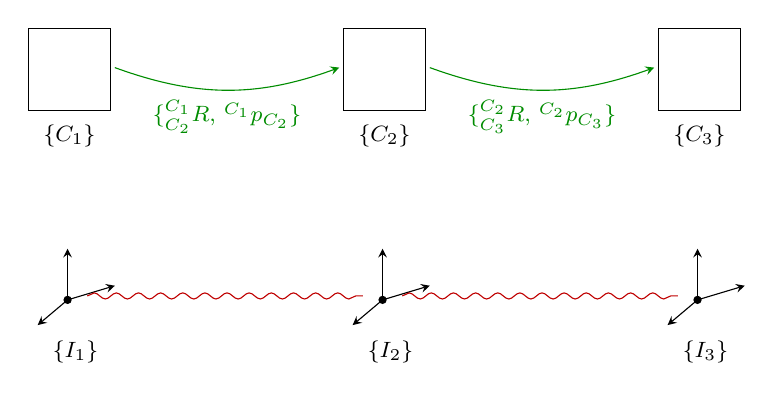
\begin{tikzpicture}[>=stealth]
  % camera frames (squares)
  \foreach \i/\x in {1/0, 2/4.0, 3/8.0} {
    \draw (\x,1.3) rectangle ++(1.05,1.05);
    \node[below] at (\x+0.525,1.25) {\footnotesize $\{C_\i\}$};
  }
  % green relative-pose links from vision
  \draw[green!55!black,->] (1.10,1.85) to[bend right=20]
    node[midway,below,font=\footnotesize] {$\{{}^{C_1}_{C_2}\vect{R},\, {}^{C_1}\vect{p}_{C_2}\}$} (3.95,1.85);
  \draw[green!55!black,->] (5.10,1.85) to[bend right=20]
    node[midway,below,font=\footnotesize] {$\{{}^{C_2}_{C_3}\vect{R},\, {}^{C_2}\vect{p}_{C_3}\}$} (7.95,1.85);
  % IMU triads
  \foreach \i/\x in {1/0.5, 2/4.5, 3/8.5} {
    \fill (\x,-1.1) circle (1.5pt);
    \draw[->] (\x,-1.1) -- ++(0,0.65);
    \draw[->] (\x,-1.1) -- ++(0.6,0.18);
    \draw[->] (\x,-1.1) -- ++(-0.38,-0.32);
    \node[below] at (\x+0.1,-1.5) {\footnotesize $\{I_\i\}$};
  }
  % red wavy IMU-integration links
  \draw[red!75!black, decorate, decoration={snake, amplitude=1.1pt, segment length=8pt}]
    (0.75,-1.05) -- (4.25,-1.05);
  \draw[red!75!black, decorate, decoration={snake, amplitude=1.1pt, segment length=8pt}]
    (4.75,-1.05) -- (8.25,-1.05);
\end{tikzpicture}
\caption{Visual-inertial initialization: the relative camera poses from the visual SLAM pipeline (top, green) are aligned with the IMU integration over the same intervals (bottom, red wavy links) through the camera--IMU extrinsics.}
\label{fig:lec06-init}
\end{figure}

From these, we want to \textbf{initialize}:
\begin{empheq}[box=\fbox]{align}
\begin{cases}
\text{(1)} & {}^{I_1}\vect{g} \\[2pt]
\text{(2)} & {}^{I_1}\vect{v}_{I_1},\; {}^{I_1}\vect{v}_{I_2},\; {}^{I_1}\vect{v}_{I_3},\; \ldots \\[2pt]
\text{(3)} & s \quad (\text{mono camera}) \\[2pt]
\text{(4)} & \vect{b}_g,\; \vect{b}_a
\end{cases}
\label{eq:lec06-init-targets}
\end{empheq}

\paragraph{From vision.} Using the visual SLAM pipeline (Lectures~3--4), we obtain the relative camera poses
\begin{align}
\big\{ {}^{C_1}_{C_2}\vect{R},\; {}^{C_1}\vect{p}_{C_2} \big\},
\qquad
\big\{ {}^{C_2}_{C_3}\vect{R},\; {}^{C_2}\vect{p}_{C_3} \big\},
\end{align}
where for a monocular camera the translations are recovered only \emph{up to a scale} $s$.

\paragraph{From IMU integration.} Recall the exact integration results of Lecture~5 (writing $\Delta\vect{p}_k, \Delta\vect{v}_k$ for the preintegrated measurements over $[t_k, t_{k+1}]$, $\delta t_k = t_{k+1} - t_k$):
\begin{align}
{}^{I_k}_{I_{k+1}}\vect{R} &= {}^{G}_{I_k}\vect{R}\trans\,{}^{G}_{I_{k+1}}\vect{R}, \\
{}^{G}\vect{p}_{I_{k+1}} &= {}^{G}\vect{p}_{I_k} + {}^{G}\vect{v}_{I_k}\,\delta t_k + {}^{G}_{I_k}\vect{R}\,\Delta\vect{p}_k + \frac{1}{2}\,{}^{G}\vect{g}\,\delta t_k^2, \\
{}^{G}\vect{v}_{I_{k+1}} &= {}^{G}\vect{v}_{I_k} + {}^{G}_{I_k}\vect{R}\,\Delta\vect{v}_k + {}^{G}\vect{g}\,\delta t_k.
\end{align}
Rotate the position update into the local frame $\{I_k\}$, defining ${}^{I_k}\vect{v}_{I_k} \triangleq {}^{G}_{I_k}\vect{R}\trans\,{}^{G}\vect{v}_{I_k}$ and ${}^{I_k}\vect{g} \triangleq {}^{G}_{I_k}\vect{R}\trans\,{}^{G}\vect{g}$:
\begin{align}
{}^{I_k}\vect{p}_{I_{k+1}}
= {}^{G}_{I_k}\vect{R}\trans\big({}^{G}\vect{p}_{I_{k+1}} - {}^{G}\vect{p}_{I_k}\big)
= {}^{I_k}\vect{v}_{I_k}\,\delta t_k + \Delta\vect{p}_k + \frac{1}{2}\,{}^{I_k}\vect{g}\,\delta t_k^2,
\label{eq:lec06-localpos1}
\end{align}
and, one interval later, expressing everything with $\{I_k\}$-frame quantities via the (gyro-integrated, hence known) rotation ${}^{I_{k+1}}_{I_k}\vect{R} = \big({}^{I_k}_{I_{k+1}}\vect{R}\big)\trans$:
\begin{align}
{}^{I_{k+1}}\vect{p}_{I_{k+2}}
&= {}^{G}_{I_{k+1}}\vect{R}\trans\big({}^{G}\vect{p}_{I_{k+2}} - {}^{G}\vect{p}_{I_{k+1}}\big)
= {}^{I_{k+1}}\vect{v}_{I_{k+1}}\,\delta t_{k+1} + \Delta\vect{p}_{k+1} + \frac{1}{2}\,{}^{I_{k+1}}\vect{g}\,\delta t_{k+1}^2 \\
&= \Delta\vect{p}_{k+1} + {}^{I_{k+1}}_{I_k}\vect{R}\left({}^{I_k}\vect{v}_{I_{k+1}}\,\delta t_{k+1} + \frac{1}{2}\,{}^{I_k}\vect{g}\,\delta t_{k+1}^2\right).
\label{eq:lec06-localpos2}
\end{align}

\paragraph{Connecting the two.} With the camera--IMU extrinsics $\{{}^{I}_{C}\vect{R}, {}^{I}\vect{p}_C\}$ (inverse $\{{}^{C}_{I}\vect{R}, {}^{C}\vect{p}_I\}$) and the monocular scale $s$ on the vision translation, chain the transformations:
\begin{align}
\begin{bmatrix}
{}^{I_k}_{I_{k+1}}\vect{R} & {}^{I_k}\vect{p}_{I_{k+1}} \\
\vect{0}_{1\times3} & 1
\end{bmatrix}
&=
\begin{bmatrix}
{}^{I}_{C}\vect{R} & {}^{I}\vect{p}_C \\
\vect{0}_{1\times3} & 1
\end{bmatrix}
\begin{bmatrix}
{}^{C_k}_{C_{k+1}}\vect{R} & s\,{}^{C_k}\vect{p}_{C_{k+1}} \\
\vect{0}_{1\times3} & 1
\end{bmatrix}
\begin{bmatrix}
{}^{C}_{I}\vect{R} & {}^{C}\vect{p}_I \\
\vect{0}_{1\times3} & 1
\end{bmatrix} \\
&=
\begin{bmatrix}
{}^{I}_{C}\vect{R}\,{}^{C_k}_{C_{k+1}}\vect{R} & s\,{}^{I}_{C}\vect{R}\,{}^{C_k}\vect{p}_{C_{k+1}} + {}^{I}\vect{p}_C \\
\vect{0}_{1\times3} & 1
\end{bmatrix}
\begin{bmatrix}
{}^{C}_{I}\vect{R} & {}^{C}\vect{p}_I \\
\vect{0}_{1\times3} & 1
\end{bmatrix} \\
&=
\begin{bmatrix}
{}^{I}_{C}\vect{R}\,{}^{C_k}_{C_{k+1}}\vect{R}\,{}^{C}_{I}\vect{R} &
{}^{I}_{C}\vect{R}\,{}^{C_k}_{C_{k+1}}\vect{R}\,{}^{C}\vect{p}_I + s\,{}^{I}_{C}\vect{R}\,{}^{C_k}\vect{p}_{C_{k+1}} + {}^{I}\vect{p}_C \\
\vect{0}_{1\times3} & 1
\end{bmatrix}.
\label{eq:lec06-handeye}
\end{align}
Hence, equating the translation of \eqref{eq:lec06-handeye} with \eqref{eq:lec06-localpos1} and \eqref{eq:lec06-localpos2}, we get the two \emph{position constraints}
\begin{align}
{}^{I}_{C}\vect{R}\,{}^{C_k}_{C_{k+1}}\vect{R}\,{}^{C}\vect{p}_I + s\,{}^{I}_{C}\vect{R}\,{}^{C_k}\vect{p}_{C_{k+1}} + {}^{I}\vect{p}_C
&= \Delta\vect{p}_k + {}^{I_k}\vect{v}_{I_k}\,\delta t_k + \frac{1}{2}\,{}^{I_k}\vect{g}\,\delta t_k^2, \\
{}^{I}_{C}\vect{R}\,{}^{C_{k+1}}_{C_{k+2}}\vect{R}\,{}^{C}\vect{p}_I + s\,{}^{I}_{C}\vect{R}\,{}^{C_{k+1}}\vect{p}_{C_{k+2}} + {}^{I}\vect{p}_C
&= \Delta\vect{p}_{k+1} + {}^{I_{k+1}}_{I_k}\vect{R}\left({}^{I_k}\vect{v}_{I_{k+1}}\,\delta t_{k+1} + \frac{1}{2}\,{}^{I_k}\vect{g}\,\delta t_{k+1}^2\right).
\label{eq:lec06-posconstraints}
\end{align}
At the same time, rotating the velocity updates into $\{I_k\}$ gives the two \emph{velocity constraints}
\begin{align}
{}^{I_k}\vect{v}_{I_{k+1}} - {}^{I_k}\vect{v}_{I_k} - {}^{I_k}\vect{g}\,\delta t_k &= \Delta\vect{v}_k, \\
{}^{I_{k+1}}_{I_k}\vect{R}\left({}^{I_k}\vect{v}_{I_{k+2}} - {}^{I_k}\vect{v}_{I_{k+1}} - {}^{I_k}\vect{g}\,\delta t_{k+1}\right) &= \Delta\vect{v}_{k+1}.
\label{eq:lec06-velconstraints}
\end{align}

\paragraph{The linear system.} Stacking the four constraints into $\vect{A}\vect{u} = \vect{b}$ with the unknowns $\vect{u} = \begin{bmatrix} s & {}^{I_k}\vect{g}\trans & {}^{I_k}\vect{v}_{I_k}\trans & {}^{I_k}\vect{v}_{I_{k+1}}\trans & {}^{I_k}\vect{v}_{I_{k+2}}\trans \end{bmatrix}\trans$ ($13\times1$), and abbreviating $\bar{\vect{R}} \triangleq {}^{I_{k+1}}_{I_k}\vect{R}$:
\begingroup
\setlength{\arraycolsep}{2pt}
\begin{empheq}[box=\fbox]{align}
\begin{bmatrix}
-{}^{I}_{C}\vect{R}\,{}^{C_k}\vect{p}_{C_{k+1}} & \tfrac{1}{2}\delta t_k^2\,\vect{I}_3 & \delta t_k\,\vect{I}_3 & \vect{0}_3 & \vect{0}_3 \\[3pt]
-{}^{I}_{C}\vect{R}\,{}^{C_{k+1}}\vect{p}_{C_{k+2}} & \tfrac{1}{2}\delta t_{k+1}^2\,\bar{\vect{R}} & \vect{0}_3 & \delta t_{k+1}\,\bar{\vect{R}} & \vect{0}_3 \\[3pt]
\vect{0}_{3\times1} & -\delta t_k\,\vect{I}_3 & -\vect{I}_3 & \vect{I}_3 & \vect{0}_3 \\[3pt]
\vect{0}_{3\times1} & -\delta t_{k+1}\,\bar{\vect{R}} & \vect{0}_3 & -\bar{\vect{R}} & \bar{\vect{R}}
\end{bmatrix}
\begin{bmatrix}
s \\ {}^{I_k}\vect{g} \\ {}^{I_k}\vect{v}_{I_k} \\ {}^{I_k}\vect{v}_{I_{k+1}} \\ {}^{I_k}\vect{v}_{I_{k+2}}
\end{bmatrix}
=
\begin{bmatrix}
{}^{I}_{C}\vect{R}\,{}^{C_k}_{C_{k+1}}\vect{R}\,{}^{C}\vect{p}_I + {}^{I}\vect{p}_C - \Delta\vect{p}_k \\[3pt]
{}^{I}_{C}\vect{R}\,{}^{C_{k+1}}_{C_{k+2}}\vect{R}\,{}^{C}\vect{p}_I + {}^{I}\vect{p}_C - \Delta\vect{p}_{k+1} \\[3pt]
\Delta\vect{v}_k \\[3pt]
\Delta\vect{v}_{k+1}
\end{bmatrix}.
\label{eq:lec06-linsys}
\end{empheq}
\endgroup
Solving this linear system recovers targets (1)--(3) of \eqref{eq:lec06-init-targets}: the scale, the gravity direction in $\{I_k\}$ (hence the initial orientation up to yaw), and the velocities.

\paragraph{How many frames do we need?} The system \eqref{eq:lec06-linsys} has $12$ constraints and $13$ unknowns. In general, every pair of consecutive frames gives $6$ constraints ($3$ position + $3$ velocity), so $n$ frames give $6(n-1)$, while we totally need to solve $1 + 3 + 3n$ unknowns ($s$, gravity, and $n$ velocities):
\begin{itemize}[noitemsep,topsep=2pt]
\item \textbf{if $s$ is known} (stereo camera): $3$ frames are good to solve the initialization;
\item \textbf{if $s$ is unknown} (mono camera):
\begin{align}
6(n-1) - (4 + 3n) > 0
\;\;\Rightarrow\;\;
n > \tfrac{10}{3}
\;\;\Rightarrow\;\;
n = 4 \;\text{frames minimum ($3$ intervals)}.
\end{align}
\end{itemize}
